
%(BEGIN_QUESTION)
% Copyright 2011, Tony R. Kuphaldt, released under the Creative Commons Attribution License (v 1.0)
% This means you may do almost anything with this work of mine, so long as you give me proper credit

In order to learn PLC programming and perform the exercises necessary for exams in this course, you must have your own PLC {\it trainer} consisting of a working PLC and input switches all wired and ready to use.  

$$\includegraphics[width=15.5cm]{i04513x01.eps}$$

All components should be securely mounted to a wood board or some other structure making it easy to transport and use.  You {\it must} have a terminal block in between the switches, indicators, and PLC I/O terminals to allow for easy connection and disconnection of external devices to your PLC without wearing out the screws on the PLC's terminal block prematurely.  Separate terminal blocks are easily replaced, whereas the terminal block on your PLC is likely much more expensive and inconvenient to replace!

Consult the user's manual for your PLC in order to determine how all devices should be wired to the input and output (I/O) terminals.  Note that often there are different types of I/O (AC, DC, sourcing, sinking) available for the same (or similar) model of PLC.  Most PLC user's manuals give detailed diagrams showing how to connect devices to discrete I/O points, so be sure to follow the proper diagram for your specific PLC model!

\vskip 10pt

Once you have your PLC wired, the next step is to install and run the software used to program your programmable logic controller (PLC), and try to get the two devices communicating with each other.  This, of course, requires you have a special cable connecting your PC to your PLC, with any necessary ``drivers'' installed on your PC to allow it to communicate.  Like all serial-based communications, the PC needs to be properly configured with regard to bit rate, number of data bits, number of stop bits, and parity in order to communicate with the PLC.  The software you will be using should have an ``auto detect'' feature which will sequentially try various combinations of these parameters until it finds one combination that works.  Note: on Allen-Bradley PLCs, you must \underbar{first} install and run software called {\it RSLinx} which manages communications between your PC and PLC, before you start up the programming software ({\it RSLogix}).

\vskip 10pt

After that, your next step is to use programming software (installed in a personal computer) to program your PLC with some simple function consisting of ``contact'' and ``coil'' instructions.  The purpose of a virtual contact in a PLC program is to {\it read} data bits from memory, while the purpose of a virtual coil in a PLC program is to {\it write} data bits to memory.  Thus, you will create programs for the PLC using virtual contacts to read the states of real-world switches connected to inputs on the PLC, and using virtual coils to control real-world outputs on the PLC to energize loads such as lamps and solenoids.  The interconnections and arrangements of these virtual contacts and coils determine the logic implemented by the PLC: specifying the conditions necessary to energize real-world devices based on input conditions.

\vskip 10pt

You will find step-by-step instructional tutorials for both Allen-Bradley MicroLogix and Koyo CLICK PLCs in your Instrumentation Reference (provided by the instructor).  Follow these tutorials to establish communication between your PC and your PLC, and to write a simple contact-and-coil ladder diagram program, before attempting the exercises that follow.  You will also find much pertinent information for programming Allen-Bradley MicroLogix PLCs in the {\it RSLogix 500 Getting Results Guide}, since the SLC 500 line of Allen-Bradley PLCs program so similarly to the MicroLogix line.

\filbreak

This example shows an Allen-Bradley MicroLogix 1000 series PLC (model 1761-L10BWA) wired to two toggle switches and one LED indicator lamp, complete with a demonstration program.  Note that line power (120 VAC) wire connections to power the PLC have been omitted, so the focus is solely on the I/O wiring:

$$\includegraphics[width=15.5cm]{i04513x02.eps}$$

Note how Allen-Bradley I/O is labeled in the program: input bits designated by the letter {\tt I} and output bits designated by the letter {\tt O}.

Based on the wiring and program you see for this PLC, identify the switch state combinations resulting in an energized lamp.  Try duplicating this program in your own PLC (even if it is a different brand or model) and see how it functions.  Be sure to activate the {\it color highlighting} feature of your programming editor so you may see the ``live'' status of the program's virtual contacts and coil!

\filbreak

This example shows a Siemens S7-200 series PLC (model 224XP) wired to two toggle switches and one LED indicator lamp, complete with a demonstration program:

$$\includegraphics[width=15.5cm]{i04513x03.eps}$$

Note how Siemens I/O is labeled in the program: input bits designated by the letter {\tt I} and output bits designated by the letter {\tt Q}.

Based on the wiring and program you see for this PLC, identify the switch state combinations resulting in an energized lamp.  Try duplicating this program in your own PLC (even if it is a different brand or model) and see how it functions.  Be sure to activate the {\it color highlighting} feature of your programming editor so you may see the ``live'' status of the program's virtual contacts and coil!

\filbreak

This example shows a Koyo ``CLICK'' PLC (model C0-02DD1-D) wired to two toggle switches and one LED indicator lamp, complete with a demonstration program:

$$\includegraphics[width=15.5cm]{i04513x04.eps}$$

Note how Koyo I/O is labeled in the program: input bits designated by the letter {\tt X} and output bits designated by the letter {\tt Y}.

Based on the wiring and program you see for this PLC, identify the switch state combinations resulting in an energized lamp.  Try duplicating this program in your own PLC (even if it is a different brand or model) and see how it functions.  Be sure to activate the {\it color highlighting} feature of your programming editor so you may see the ``live'' status of the program's virtual contacts and coil!




\underbar{file i04513}
%(END_QUESTION)





%(BEGIN_ANSWER)

For the Allen-Bradley MicroLogix example, the lamp will energize only when switch 0 is turned off and switch 1 is turned on.

\vskip 10pt

For the Siemens S7-200 example, the lamp will energize when switch 0 is turned on or if switch 1 is turned off, or both conditions occur simultaneously.

\vskip 10pt

For the Koyo example, the lamp will energize according to the {\it Exclusive-OR} function with switch 1 and switch 2.  The lamp energizes when switch 1 is on and switch 2 is off, or when switch 1 is off and switch 2 is on.

%(END_ANSWER)





%(BEGIN_NOTES)

It is recommended that the instructor note which brand and model of PLC each of their students uses to build their trainer.  Future assessments will require students program PLCs {\it different} from their own!

\vskip 20pt \vbox{\hrule \hbox{\strut \vrule{} {\bf Virtual Troubleshooting} \vrule} \hrule}

This question is a good candidate for a ``Virtual Troubleshooting'' exercise.  Presenting the diagram to students, you first imagine in your own mind a particular fault in the system.  Then, you present one or more symptoms of that fault (something noticeable by an operator or other user of the system).  Students then propose various diagnostic tests to perform on this system to identify the nature and location of the fault, as though they were technicians trying to troubleshoot the problem.  Your job is to tell them what the result(s) would be for each of the proposed diagnostic tests, documenting those results where all the students can see.

During and after the exercise, it is good to ask students follow-up questions such as:

\begin{itemize}
\item{} What does the result of the last diagnostic test tell you about the fault?
\item{} Suppose the results of the last diagnostic test were different.  What then would that result tell you about the fault?
\item{} Is the last diagnostic test the best one we could do?
\item{} What would be the ideal order of tests, to diagnose the problem in as few steps as possible?
\end{itemize}

%INDEX% PLC, building a "trainer"

%(END_NOTES)

